\section{User Interface}

\subsection{General Purpose Tools}
\begin{figure}[H]
\centering

\includegraphics[scale=0.65]{fig/MainToolbar}
\caption{General purpose toolbar.}
\end{figure}

These tools offer basic funcionality independent of any specific context.\\

\vspace{0.3cm}
%\desc{Show Segmentations}{../../frontend/rsc/show_all}
%{Segmentations are shown in planar views}
\begin{tabular}{| m{1.3cm} | m{12cm} |}
\hline
\textbf{Button} & \textbf{Description}\\
\hline
& Visibility button is a toggle button with two states.\\ 

\includegraphics[width=0.6cm]{../../frontend/rsc/show_all} &
\textbf{Show Segmentations}: All segmentations are shown in planar views.\\

\includegraphics[width=0.6cm]{../../frontend/rsc/hide_all} &
\textbf{Hide Segmentations}: All segmentations are hidden in planar views.\\
\hline
& Crosshair button is a toggle button with two states.\\ 

\includegraphics[width=0.6cm]{../../frontend/rsc/show_planes} &
\textbf{Show Crosshair}: Crosshair is shown in planar views.\\
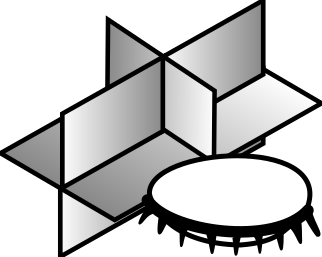
\includegraphics[width=0.6cm]{../../frontend/rsc/hide_planes} &
\textbf{Hide Crosshair}: Crosshair is hidden in planar views.\\
\hline
 & %No icon
\textbf{Taxonomy Selector}: Some tools may require the user to specify a
taxonomy label to be applied when segmentations are created.\\
\hline

\includegraphics[width=0.6cm]{../../frontend/rsc/removeSeg} &
\textbf{Delete Segmentation}: Deletes segmentations by clicking on them on one of the planar views.\\
\hline
\end{tabular}

\subsection{Volume Of Interest}

It's a volume to limit the effect of other tools, so the tool algorithm will not
go farther than the boundaries that define the volume.\\

To use it, just click on the toolbar button an then left click on the center of
the view area you want to place the volume of interest. Once the volume has been
placed the user can modify it's dimensions by clicking and dragging on the edges.\\

Only a volume of interest can be applied at a given time.\\

\vspace{0.3cm}
\begin{tabular}{| m{1.3cm} | m{12cm} |}
\hline
\textbf{Button} & \textbf{Description}\\
\hline

\includegraphics[width=0.6cm]{../../frontend/toolbar/voi/rsc/roi} &
\textbf{Rectangular Cuboid}: Define an axis aligned rectangular cuboid as volume
of interest.\\
\hline
\end{tabular}

\subsection{Channel Explorer}
Display all channels, grouped by physical sample, that are currently
loaded.Channel visibility can be toggled by clicking on the \textit{eye} icon on
the left of channels.Certain \espina's tools may require selecting channel in
order to be used. These tools will use the active channel. Active channels are
displayed in bold font in Channel Explorer.

\begin{figure}[H]
\centering
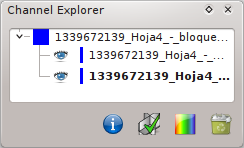
\includegraphics{fig/ChannelExplorer}
\caption{Channel explorer widget.}
\end{figure}

\begin{tabular}{| m{1.3cm} | m{12cm} |}
\hline
\textbf{Button} & \textbf{Description}\\
\hline
 & \textbf{Spacing Information}: Modify channel's spacing.\\
\hline

\includegraphics[width=0.6cm]{../../frontend/rsc/activeChannel} &
\textbf{Activate Channel}: Mark selected channel as active channel. Operations
are always applied to the active channel independently whether they are visible
or not.\\
\hline

\includegraphics[width=0.6cm]{../../frontend/rsc/rainbow} &
\textbf{Change Stain}: Display stain color selector for selected channel.\\
\hline

\includegraphics[width=0.6cm]{../../frontend/rsc/trash-full} &
\textbf{Unload Channel}: Unload current channel from \espina. The channel itself
is not modified nor deleted from disk.\\
\hline
\end{tabular}
\vspace{0.3cm}

\subsection{Taxonomy Explorer}
Display available taxonomy elements. Users can create new taxonomy's elements,
modify or delete existing ones.
\begin{figure}[H]
\centering
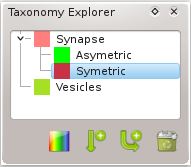
\includegraphics{fig/TaxonomyExplorer}
\caption{Taxonomy explorer widget.}
\end{figure}

\begin{tabular}{| m{1.3cm} | m{12cm} |}
\hline
\textbf{Button} & \textbf{Description}\\
\hline

\includegraphics[width=0.6cm]{../../frontend/rsc/rainbow} &
\textbf{Change Color}: Display a color selector window to change the color
assoicated with selected taxonomy.\\
\hline

\includegraphics[width=0.6cm]{../../frontend/rsc/create_node} &
\textbf{Add Taxonomy}: Create a new segmentation at the same level than the
selected one.\\
\hline

\includegraphics[width=0.6cm]{../../frontend/rsc/create_subnode} &
\textbf{Add SubTaxonomy}: Create a new segmentation as a child of the selected
one.\\
\hline

\includegraphics[width=0.6cm]{../../frontend/rsc/remove} &
\textbf{Delete Taxonomy}: Delete selected taxonomy. Only taxonomies which are
not in use can be deleted.\\
\hline
\end{tabular}
\vspace{0.3cm}

\subsection{Segmentation Explorer}
Display all segmentations that are currently loaded. Segmentation visibility can
be toggled by clicking on the \textit{eye} icon on the left of segmentations.
\begin{figure}[H]
\centering
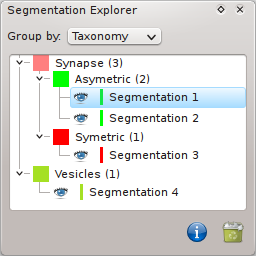
\includegraphics{fig/SegmentationExplorer}
\caption{Segmentation explorer widget.}
\end{figure}

Segmentations can be arranged using different grouping critearias:
\begin{itemize}
  \item None Display a list with all segmentations.
  \item Taxonomy Display each segmentation under their corresponding taxonomy
element.
  \item Sample Display each segmentation under their corresponding sample.
\end{itemize}
\vspace{0.3cm}

\begin{tabular}{| m{1.3cm} | m{12cm} |}
\hline
\textbf{Button} & \textbf{Description}\\
\hline
 & %No icon
\textbf{Segmentation Information}: Open the segmentation inspectors for the
selected segmentations.\\
\hline

\includegraphics[width=0.6cm]{../../frontend/rsc/trash-full} &
\textbf{Delete Segmentation}: Delete selected segmentations. When a grouping
element is selected, recursive deletion is available.\\
\hline
\end{tabular}
\vspace{0.3cm}

\subsubsection{Segmentation Inspector}
Display all available information of a segmentation. Available 3D
representations can be displayed using the three-dimensioanl view. Information
about the creation of the segmentation is displayed in the filter inspector on
the right side of the window. Finally, all available information is displayed
in the segementation information data table under the three-dimensional view.

\begin{figure}[H]
\centering
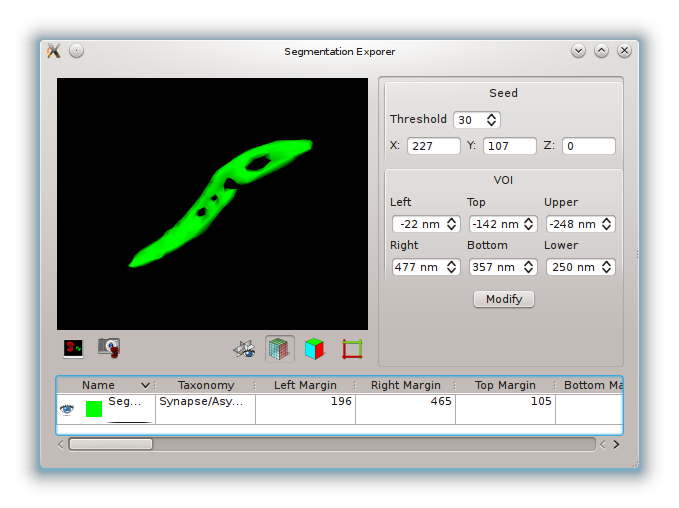
\includegraphics[width=\linewidth]{fig/SegmentationInspector}
\caption{Segmentation inspector widget.}
\end{figure}

For more specific information of each component, please refer to the
corresponding section.

\subsection{Filter Inspector}
The filter inspector shows relevant information about the filter that created the segmentation,
therefore the information shown is dependent on the filter or plugin filter used.

\begin{figure}[H]
\centering
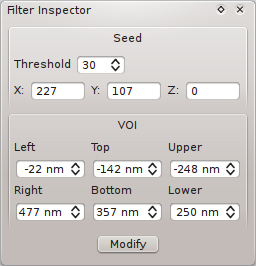
\includegraphics{fig/SeedGrowSegmentationFilterInspector}
\caption{Filter inspector widget showing the information of a seed grow filter.}
\end{figure}
